\begin{wrapfigure}{r}{0.5\textwidth}%
\centering%
\vspace{-1cm}
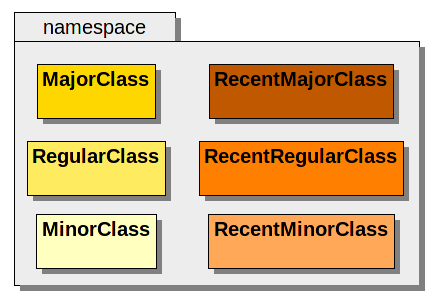
\includegraphics[scale=.33]{../classdiagrams/uml-legend.png}%
\caption{Color conventions in UML diagrams.}%
\label{fig:uml-legend}%
\end{wrapfigure}%

\section{Introduction}

This chapter present the design of \sofa{}, as well as its recent evolutions.
It also includes discussions justifying some of the decision that are behind this design.

The conventions used in UML class diagrams are presented in Fig~\ref{fig:uml-legend}.

\vspace{.8cm}

\section{Core Class Diagrams}

\subsection{Object Model (\textcode{sofa::core::objectmodel})}

\begin{figure}[h]
\centering
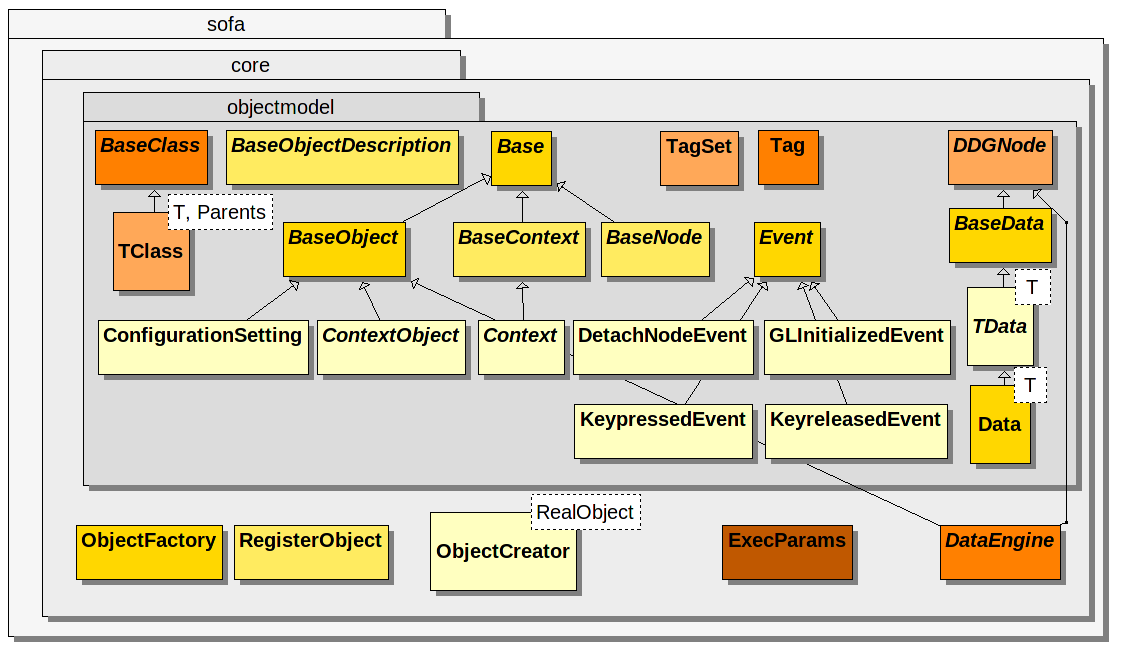
\includegraphics[scale=.33]{../classdiagrams/sofacore-objectmodel.png}
\caption{Classes of the \textcode{sofa::core::objectmodel} namespace.}
\label{fig:uml-sofa-core-objectmodel}
\end{figure}

\subsubsection{Changes compared to the 1.0~beta~4 version}\label{sec:design-core-objectmodel-changes}

\paragraph{New class description system.}
It is based on the \textcode{BaseClass} and \textcode{TClass} classes, and requires to add the \textcode{SOFA\_CLASS} macro in the declaration of all classes deriving from Base.
The benefits are that it is now possible to follow the full hierarchy of classes from the final components, instead of having just a fixed set of categories.
This macro is also necessary in classes with a templated parent class to be able to use methods and member variables defined in \textcode{Base} such as \textcode{initData} or \textcode{sout}. This removed all the previously redundant direct heritage to \textcode{BaseObject} that was previously required.

\paragraph{Objects and node tagging (\textcode{Tag} and \textcode{TagSet}).}
The goal of the introduction of tags is to provide one of the pieces necessary to support non-mechanical states (electrical potentials, constrast agent concentrations) as well as cleaner non-geometrical mechanical states (fluid dynamics, reduced-coordinate articulations).
For example, in a simulation involving blood in deformable vessels, we would use two tags to distinguish the different states : mechanical, fluid.
These tags will be used to easily work with only a subset of the components, so that the mechanical solver works on positions and forcefields but don't interferes with blood flow and pressure, and inversely for the fluid solver (see \footnote{http://wiki.sofa-framework.org/tdev/wiki/Notes/ProposalGenericStates} ).
We decided on using there tags instead of extending the class hierarchy as was done before with the \textcode{State} and \textcode{MechanicalState} classes.
A hierarchy is fine when we have only one feature that we want to differentiate on (such as base vs mechanical vs electrical), but when we add other criteria (lagrangian geometry vs eulerian vs reduced generalized coordinates, velocity vs vorticity, independent vs mapped DOFs) it is no longer manageable as specialized classes.
A secondary use of these tags is to replace existing subsets mechanisms within CollisionModels (r2441) and Constraints (r3121).
The design is based on the following elements.
Tags are added to BaseObject, as a list of string (internally converted to a list of unique ids for faster processing).
All visitors now filter the objects they process based on their list of tags.
All solvers by default copy their own list of tags to the visitors they execute, so that they only affect the objects with the same tags as they have (TODO: this is currently broken). 

\paragraph{Dependencies between Data (\textcode{DDGNode} and \textcode{DataEngine}).}
The goal is to be able to specify simple links between datas or through computation engines.
To function correctly, the methods \textcode{getValue()} or \textcode{beginEdit()}/\textcode{endEdit()} are required to be called in all codes accessing values contained in Data instances.
To enforce this, the class DataPtr was removed.
Note also that it is very inefficient to call \textcode{getValue()} repetively within computation loops.
Instead, the recommanded method is to use the helper classes \textcode{ReadAccessor} and \textcode{WriteAccessor}
that can hold a reference to a \textcode{Data} value, provides the same API as regular vectors,
and automatically calls \textcode{endEdit()} at the end of the call block in case of \textcode{WriteAccessor}.

\textbf{TODO:} \textit{\textcode{TData<T>} was useful as a common parent for \textcode{Data<T>} and \textcode{DataPtr<T>}, but now that \textcode{DataPtr} no longer exist, it would simplify the hierarchy to merge \textcode{TData<T>} and \textcode{Data<T>}.}

\paragraph{\textit{Copy-on-Write} (CoW) mechanism (\textcode{DataContainer}).}
The goal is to reduce copies of datas when using engines and/or multi-threading.
It is completly transparent to other codes, since everything should now respect the data access API (see above).
There is however one important side-effect that may break some existing code: the pointer to the value of a \textcode{Data} can now change during a call to \textcode{beginEdit()}.
This means that it is now illegal to retrieve the pointer to the value in a \textcode{Data} at init time and then reuse it after edits might have been made.

\paragraph{Support for asynchronous multi-threading (\textcode{ExecParams}).}
This feature is an important goal of the new design, however it is not yet completely functionnal and thus may change shortly.


\subsection{Physical Behavior (\textcode{sofa::core::behavior})}
\begin{figure}[h]
\centering
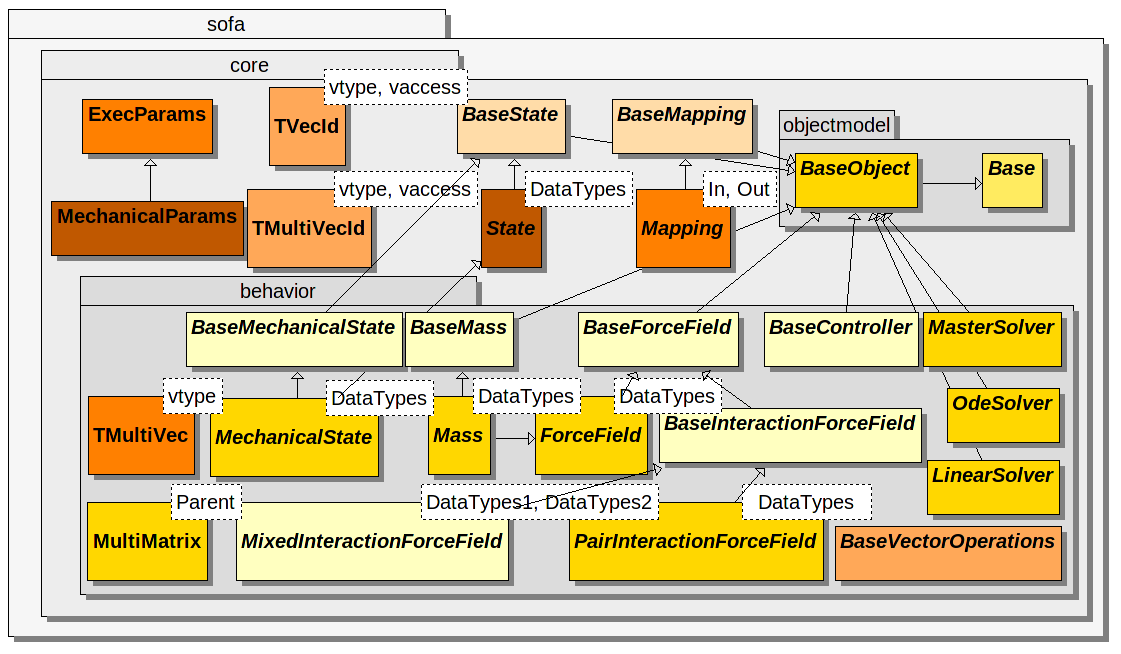
\includegraphics[scale=.33]{../classdiagrams/sofacore-behavior.png}
\caption{Classes of the \textcode{sofa::core::behavior} namespace.}
\label{fig:uml-sofa-core-behavior}
\end{figure}

\subsubsection{Changes compared to the 1.0~beta~4 version}\label{sec:design-core-behavior-changes}

\paragraph{\textcode{VecId} is replaced by templated classes to specify vector types and read/write access.}

Previously, the \textcode{VecId} class was used by solvers and visitors to specify on which state vectors should an operation be applied.
However, this API did not express the requirements for these vectors (which type, i.e. \textcode{Coord}, \textcode{Deriv}, or \textcode{MatDeriv}), nor if they were supposed to be read or written.
Now, methods and visitors can use the following classes instead (all typedefs from a common \textcode{TVecId} templated class), so that developers will now explicitly what to expect:

\begin{code_cpp}
/// Identify one vector stored in State
/// A ConstVecId only provides a read-only access to the underlying vector.
typedef TVecId<V_ALL, V_READ> ConstVecId;

/// Identify one vector stored in State
/// A VecId provides a read-write access to the underlying vector.
typedef TVecId<V_ALL, V_WRITE> VecId;

/// Typedefs for each type of state vectors
typedef TVecId<V_COORD, V_READ> ConstVecCoordId;
typedef TVecId<V_COORD, V_WRITE>     VecCoordId;
typedef TVecId<V_DERIV, V_READ> ConstVecDerivId;
typedef TVecId<V_DERIV, V_WRITE>     VecDerivId;
typedef TVecId<V_MATDERIV, V_READ> ConstMatrixDerivId;
typedef TVecId<V_MATDERIV, V_WRITE>     MatrixDerivId;
\end{code_cpp}

Also, a new class \textcode{TMultiVecId} is introduced to be able to specify different IDs for specific states or groups of states. Similar typedefs are defined as above, replacing \textcode{Vec} with \textcode{MultiVec}.

\paragraph{New State API and class hierarchy.}
The previous State API was based on \textcode{getX()}/\textcode{getV()}/... methods that returned pointers to the vectors last specified (using \textcode{setX()}/\textcode{setV()}/... methods) as the current position, velocity, ...
This is now replaced by \textcode{read(ConstVec\textit{TYPE}Id)} and \textcode{write(Vec\textit{TYPE}Id)} methods, where \textcode{\textit{TYPE}} is either \textcode{Coord}, \textcode{Deriv}, or \textcode{MatDeriv}.
These methods return a pointer to a Data instance containing the vector, instead of the vector itself.
This was necessary to respect the Data access API (see section~\ref{sec:design-core-objectmodel-changes}).
For compatibility with existing codes (especially \textcode{draw()} methods), the read-only \textcode{getX()}/\textcode{getV()}/... methods still exists but they are deprecated (and there are strictly equivalent to calling \textcode{read()} with the default ID for position, velocity, ...).
The non-const versions however are removed, so all codes modifying state vectors will have to use the new Data-based API.
Note that with this change, the state components no longer store the information about which vectors should be considered as the current position, velocity, ...
So another mechanism is required to specify these associations (\textcode{MechanicalParams}, see below).

A new state class hierarchy is also defined,  introducing a new parent class \textcode{BaseState}, common to all states (mechanical, visual, ...).
Methods allowing to read and write vectors given their IDs are specified in \textcode{State<DataTypes>}.
The \textcode{MappedModel} class is removed, non-mechanical state components (such as visual models) now directly derive from \textcode{State<DataTypes>}.


\paragraph{Simplified \textcode{Mapping} class hierarchy.}
Previously, a different base class (\textcode{Mapping< State<TIn>, MappedModel<TOut> >} or \textcode{MechanicalMapping< MechanicalState<TIn>, MechanicalState<TOut> >}) where used for mechanical versus non-mechanical (i.e. visual or one-way) mappings.
This introduced complexities and redundancies in the code of the final components (they where templated by the type of their parent class and compiled twice for each pair of input/output datatypes).
Now, a single base class is used (\textcode{Mapping<TIn,TOut>}, templated only by the input and output datatypes.
Components are also templated by the same types, similarly to other classes such as forcefields.
A new set of flags is used to check if a given mapping is mechanical or not.
Different flags are used to activate the mapping of forces, masses, and constraints separatly (although by default they have the same value).
Components that do not implement applyJT (i.e. visual mappings) can force them to false to indicate they do not support mechanical computations.

\paragraph{New mechanical component API based on \textcode{Data} and \textcode{MechanicalParams}.}
This is the most important change from the previous design.
To provide all the required vector IDs that where previously stored within each \textcode{MechanicalState} by calls to \textcode{setX()}/... methods, we define a \textcode{MechanicalParam} class.
This class is given to all mechanical-related methods, specified by \textcode{OdeSolver}s and transmitted by \textcode{MechanicalVisitor}s.
It hides the \textcode{VecId} system from most component codes, providing the same abstraction of accessing the current position and velocity vectors as was previously handled within \textcode{MechanicalState}. For example, where a component such as a \textcode{ForceField} implementation used :
\begin{code_cpp}
const VecCoord* x = this->mstate->getX();
\end{code_cpp}
It will now use \textcode{MechanicalParams} as follows :
\begin{code_cpp}
helper::ReadAccessor<VecCoord> x = *mparams->readX(this->mstate);
\end{code_cpp}

This API is preferable to directly manipulating \textcode{VecId}s (such as in \textcode{this->mstate->read(mparams->getXId(this->mstate))}) because :
\begin{itemize}
\item The code is very similar to the previous version.
\item If the API of the \textcode{VecId} or \textcode{MechanicalState} class is further changed, the \textcode{MechanicalParam::readX()} method can handle it.
\item Different \textcode{VecId}s for different states can be chosen within \textcode{MechanicalParam} (such as what is currently used for free vs mapped states, and animated vs external obstacle state).
\end{itemize}

However it is still possible to get the ids (using \textcode{mparams->x().getId(mstate)}).

All vector accesses given though \textcode{MechanicalParams} are read-only.
Vectors actually modified by each method are given as separate \textcode{MultiVecId} parameters.
This is useful to make the API clearer (we can see explicitly what each method is supposed to write) and safer (no accidental modifications to X or V within \textcode{addForce()} or \textcode{draw()} for example).
Finally, other interesting pieces of information can be queried though \textcode{MechanicalParams}.
For example, a ForceField can know as soon as the \textcode{addForce()} call if the current solver is implicit or explicit, if the kinematic and potential energy should be computed, ...

\paragraph{New solver hierarchy and vector manipulation API (\textcode{TMultiVec} and \textcode{BaseVectorOperations}).}
Previously, the solver classes had a complex hierarchy, with several parent classes (\textcode{SolverImpl}, \textcode{OdeSolverImpl}, \textcode{MasterSolverImpl}) that where used to launch each type of visitors (mechanics, linear algebra, ...).
In the new design, these classes are replaced by separate helper classes (\textcode{VectorOperations}, \textcode{MechanicalOperations}) that are instanciated at runtime and allow to launch each type of visitors while holding and updating the persistant parameters (in the form of a \textcode{MechanicalParams} for mechanical visitors for example, or \textcode{ExecParams} for simple vector operations).


\subsection{Topology (\textcode{sofa::core::topology})}

\textit{The design of this namespace is still a work in progress, so major changes should still be expected...}

\subsubsection{Changes compared to the 1.0~beta~4 version}

\textit{To be documented...}

\subsection{Collision (\textcode{sofa::core::collision})}

\begin{figure}[h]
\centering
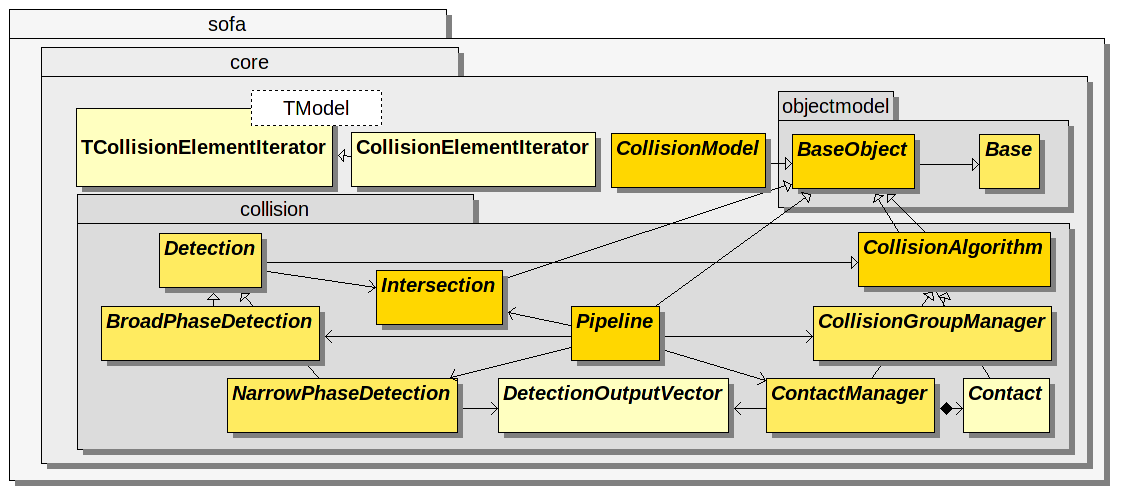
\includegraphics[scale=.33]{../classdiagrams/sofacore-collision.png}
\caption{Classes of the \textcode{sofa::core::collision} namespace.}
\label{fig:uml-sofa-core-collision}
\end{figure}

\subsubsection{Changes compared to the 1.0~beta~4 version}

\textit{No major changes.}

\subsection{Mesh and Image Loaders (\textcode{sofa::core::loader})}

\begin{figure}[h]
\centering
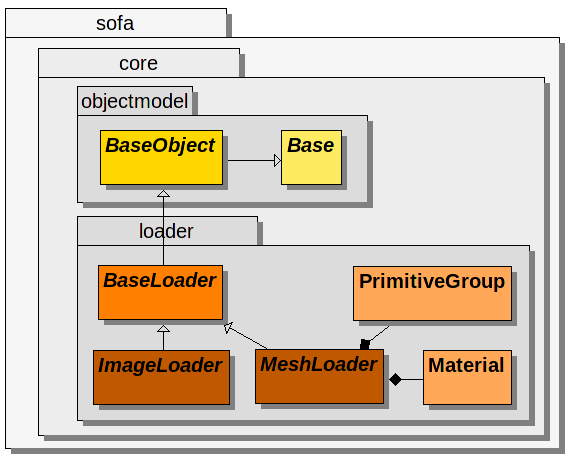
\includegraphics[scale=.33]{../classdiagrams/sofacore-loader.png}
\caption{Classes of the \textcode{sofa::core::loader} namespace.}
\label{fig:uml-sofa-core-loader}
\end{figure}

\subsubsection{Changes compared to the 1.0~beta~4 version}

This namespace is completely new.

\textit{To be documented...}

\pagebreak

\section{Main classes}

\subsection{\textcode{sofa::core::objectmodel}}

\subsubsection{\textcode{Base}}

\lstinputlisting[style=C++,linerange=51-181]{../../framework/sofa/core/objectmodel/Base.h}

\subsubsection{\textcode{BaseObject}}

\lstinputlisting[style=C++,linerange=61-160]{../../framework/sofa/core/objectmodel/BaseObject.h}

\subsection{\textcode{sofa::core}}

\subsubsection{\textcode{BaseState}}

\lstinputlisting[style=C++,linerange=39-58]{../../framework/sofa/core/BaseState.h}

\subsubsection{\textcode{State}}

\lstinputlisting[style=C++,linerange=38-103]{../../framework/sofa/core/State.h}

\subsubsection{\textcode{BaseMapping}}

\lstinputlisting[style=C++,linerange=48-116]{../../framework/sofa/core/BaseMapping.h}

\subsubsection{\textcode{Mapping}}

\lstinputlisting[style=C++,linerange=43-115]{../../framework/sofa/core/Mapping.h}


%% \section{Framework}

%% \subsection{UML Diagrams}

%% \begin{figure}[h]
%% \centering
%% 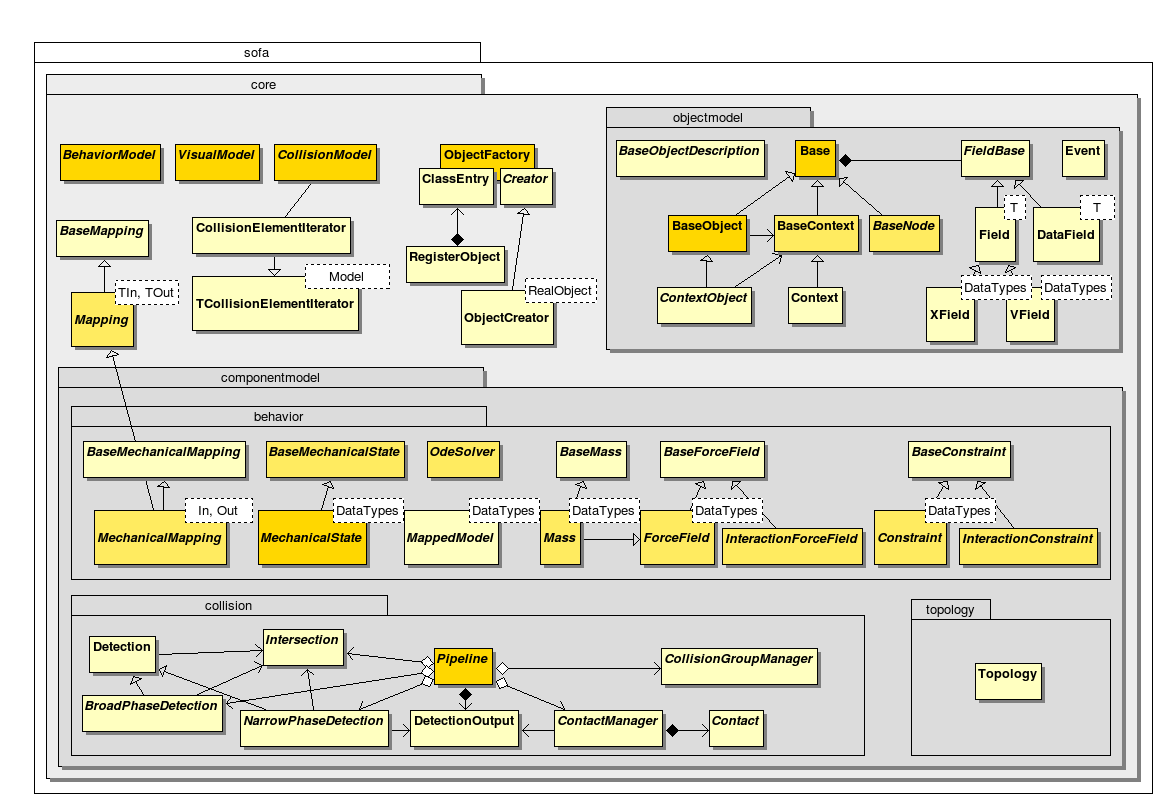
\includegraphics[width=\linewidth]{uml-sofa-core.png}
%% \caption{Classes of the sofa::core namespace.}
%% \label{fig:uml-sofa-core}
%% \end{figure}
